\begin{center}
\large Experimento: \textbf{Integradores e diferenciadores usando amplificadores operacionais}
\end{center}

\setlength{\abovedisplayskip}{-10pt}
\setlength{\belowdisplayskip}{-10pt}

\section{Introdução}

O presente relatório visa detalhar o experimento laboratorial realizado na disciplina laboratório de circuitos eletrônicos no dia 08 de outubro de 2019 sobre o assunto de integradores e diferenciadores utilizando amplificadores operacionais (AMPOPs), mais especificamente os do circuito integrado LF353. Com o objetivo de compreender o funcionamento dos circuitos integradores e diferenciadores analógicos usando AMPOPs. Os esquema dos circuitos analisados são mostradas abaixo.

\begin{figure}[H]
\begin{center}
\begin{tikzpicture}[scale=0.9]
    %shorts
    \draw (0,0) node[op amp] (opamp) {}
    (opamp.+) to[short,-] (-1.5,-0.55) to[R, l_=$R_B$] (-1.5,-2.5)
    (opamp.-) to[R,l_=$R_1$,-*] (-4,0.5) node[left] {$V_{in}$}
    (opamp.out) --  (2,0) node[right] {$V_o$}
    (opamp.up) --++(0,0.25) node[vcc]{15\,\textnormal{V}}
    (opamp.down) --++(0,-0.25) node[vee]{-15\,\textnormal{V}}
    %(-1.16,0.49) to[R,l_=$R_1$,-*] (-4,0.49) node[left] {$V_{in}$}
    (-1.5,0.5) to[short,*-] (-1.5,2.5)
    (1.5,0) to[short,*-] (1.5,2.5)
    (1.5,2.5) to[R,l_=$R_f$,-] (-1.5,2.5)
    (1.5,4) to[C,l_=$C_1$,-] (-1.5,4)
    (1.5,4) to[short,-*] (1.5,2.5)
    (-1.5,4) to[short,-*] (-1.5,2.5)
    %(-1.5,-0.50) to[R, l_=$R_B$] (-1.5,-2.5)
    (1.5,0) to[R, l=$R_L$] (1.5,-2.5)
    (-1.5,-2.5) node[ground]{} 
    (1.5,-2.5) node[ground]{} 
    ;
\end{tikzpicture}

\end{center}
\caption{Integrador.}
\label{ckt:1} 
\end{figure}




\begin{figure}[H]
\begin{center}
\begin{tikzpicture}
    %shorts
    \draw (0,0) node[op amp] (opamp) {}
    (opamp.+) -- (-1.5,-0.5)
    (opamp.-) to[C,l_=$C_2$,-] (-3.5,0.5) 
    (opamp.out) --  (2,0) node[right] {$V_o$}
    (opamp.up) --++(0,0.25) node[vcc]{15\,\textnormal{V}}
    (opamp.down) --++(0,-0.25) node[vee]{-15\,\textnormal{V}}
    %(-1.16,0.49) to[R,l_=$R_1$,-*] (-4,0.49) node[left] {$V_{in}$}
    (-1.5,0.5) to[short,*-] (-1.5,2.5)
    (1.5,0) to[short,*-] (1.5,2.5)
    (1.5,2.5) to[R,l_=$R_f$,-] (-1.5,2.5)
    (-1.5,-0.49) to[R, l_=$R_B$] (-1.5,-2.5)
    (1.5,0) to[R, l=$R_L$] (1.5,-2.5)
    (-1.5,-2.5) node[ground]{} 
    (1.5,-2.5) node[ground]{} 
    (-3.5,0.5) to[R,l_=$R_1$,-] (-6,0.5) node[left] {$V_{in}$}
    ;
\end{tikzpicture}

\end{center}
\caption{Derivador.}
\label{ckt:2} 
\end{figure}

Os circuitos integradores e diferenciadores como o próprio nome já diz, realizam a operação de integração e derivação para os sinais de entradas (formas de onda) aplicadas neles. O circuito integrador, em si, fornece na saída uma diferença de potencial que é proporcional a área sob a curva que define o sinal. Já o circuito diferenciador é basicamente um detector da taxa de variação do sinal de entrada em relação ao tempo. Podemos ver na figura 1 e 2, respectivamente, exemplos utilizando AMPOP para de circuito integrador e diferenciador. 

A atividade nos mostra dois circuitos, um integrador prático e um diferenciador prático, ela foi dividida em duas parte, uma na análise em frequência de ambos circuitos, com a medição da magnitude e fase para frequências entre 1Hz e 100kHz, além da frequência de corte. A outra parte da atividade experimental se trata na análise comparativa da saída aplicando uma onda quadrada na entrada para três frequências diferentes, uma muito menor que a frequência de corte, uma muito maior e outra na frequência de corte de ambos sistemas. 

O osciloscópio digital foi utilizado para medir as formas de onda na entrada e na saída do amplificador de instrumentação, como forma de comparar os valores e comprovar os resultados teóricos.


\section{Análise Teórica}

\subsection{Integrador}

Reconhece-se a função de transferência para o integrador prático do circuito da figura \ref{ckt:1} como:

\begin{center}
\begin{equation} \label{tip}
        T_{IP}(s) = - \frac{\frac{R_F}{R_1}}{1+\frac{s}{\frac{1}{R_FC}}} =  \frac{k_i}{1+\frac{s}{\omega_{ci}}}
\end{equation}
\end{center}

Comparando a igualdade da equação \ref{tip} pode-se determinar os parâmetros de ganho e de frequência de corte para o integrador, podendo serem encontrados por:

\begin{center}
\begin{equation} \label{tip:1}
         k_i = - \frac{R_F}{R_1} = -10
\end{equation}
\end{center}

\begin{center}
\begin{equation} \label{tip:2}
       \omega_{ci} = 2 \pi f_{ci} = \frac{1}{R_FC_1} = 2 \pi 1061 rad/s
\end{equation}
\end{center}

Assim permite-se identificar a frequência de corte $f_{ci}$ do integrador como $1.061kHz$.

Em termos de tensão de entrada e saída, para observar os efeitos do circuito em torno da frequência de corte, pode-se injetar na entrada do circuito uma tensão na forma:

\begin{center}
\begin{equation} \label{int:1}
       v_i(t) = sen(\omega_{ci}t) V
\end{equation}
\end{center}

Nessa região espera-se que o ganho da função de transferência, bem como o ângulo de defasagem sejam:

\begin{center}
\begin{equation} \label{int:1}
       |T_{ip}(\omega_{ci})| = |k_i| \times 0.707 = 7.07 V/V
\end{equation}
\end{center}

\begin{center}
\begin{equation} \label{int:2}
       \angle T_{ip}(\omega_{ci})  = 135°
\end{equation}
\end{center}

Assim a saída será:

\begin{center}
\begin{equation} \label{int:3}
       v_o(t) = |T_{ip}(\omega_{ci})| \times |v_i(t)| \times sen(\omega_{ci}t + T_{ip}(\omega_{ci})) = 7.07\times sen(\omega_{ci}t + 135°) V
\end{equation}
\end{center}

Dessa forma, a resposta em frequência pode ser observada a partir dos diagramas de bode da função de transferência. A curva de módulo indica um perfil de integração quase ideal para frequências maiores que a de corte e atribui um ganho finito para frequências abaixo daquela. A curva de ângulo mostra que o integrador é inversor.

Se injetado um sinal quadrado no integrador cujo o espectro de frequência possui harmônicas, pode-se perceber que de acordo com que a faixa de frequências de maior potência fique a frequências acima da de corte, haverá uma intensa integração do sinal, resultando em uma função triangular na saída. Porém, de acordo com que as frequências do sinal diminuam, elas enfrentarão a região de ganho constante, com apenas poucas frequências sendo integradas. Mas já que o espectro de frequência de um sinal limitado no tempo é infinito, as harmônicas de maior frequência e menor potência serão integradas, implicando em um sinal de saída que não será perfeitamente quadrado, mesmo que as frequências principais do sinal se encontrem em baixas frequências.

\begin{figure}[H]
\begin{center}
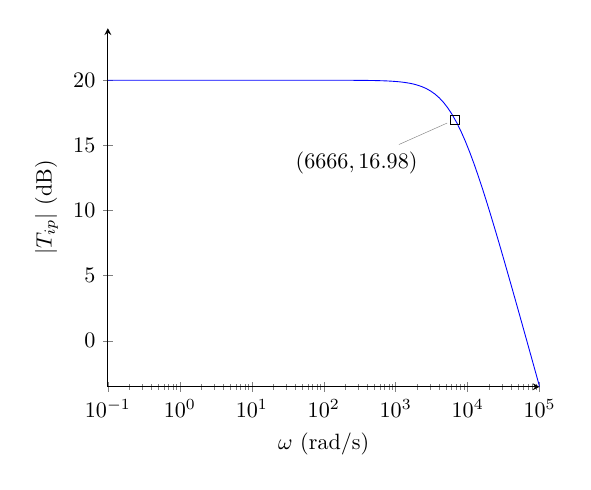
\begin{tikzpicture} [scale=0.8]
\begin{semilogxaxis}[
    axis lines = left,
    xlabel = {$\omega$ (rad/s)},
    ylabel = {$|T_{ip}|$ (dB)},
]
\addplot [
    domain=0.1:10000, 
    samples=100, 
    color=white,
]
{24*log10(10/sqrt(1+(x/6666)^2))};
\addplot [
    domain=0.1:100000, 
    samples=100, 
    color=blue,
]
{20*log10(10/sqrt(1+(x/6666)^2))};
\addplot[mark=square] coordinates {(6666,16.98)} node[pin=220:{$(6666,16.98)$}]{};
\end{semilogxaxis}
\end{tikzpicture}
\hspace{1cm}
\begin{tikzpicture} [scale=0.8]
\begin{semilogxaxis}[
    axis lines = left,
    xlabel = {$\omega$ (rad/s)},
    ylabel = {$\angle T_{ip} $ (°)},
    xtick={10,100,1000,10000,100000,1000000,10000000},
    ytick={180, 135, 90, 0},
]
\addplot [
    domain=10:10000000, 
    samples=100, 
    color=blue
]
{180-atan(x/(6666))};
\addplot[mark=square] coordinates {(6666,135)} node[pin=220:{$(6666,135)$}]{};
\addplot [
    domain=10:10000000, 
    samples=100, 
    color=white
]
{180};
\addplot [
    domain=10:10000000, 
    samples=100, 
    color=white
]
{90};
\end{semilogxaxis}
\end{tikzpicture}
\end{center}
\caption{Curvas de bode teóricas da função de transferência do integrador.}
\label{bode:1} 
\end{figure}



\subsection{Derivador}

Reconhece-se a função de transferência para o derivador prático do circuito da figura \ref{ckt:2} como:

\begin{center}
\begin{equation} \label{tdp}
        T_{DP}(s) = - \frac{s\frac{R_F}{R_1}}{s+\frac{1}{R_1C}} =  \frac{sk_d}{s+\omega_{cd}}
\end{equation}
\end{center}

Comparando a igualdade da equação \ref{tdp} pode-se determinar os parâmetros de ganho e de frequência de corte para o derivador, podendo serem encontrados por:

\begin{center}
\begin{equation} \label{tdp:1}
         k_d = - \frac{R_F}{R_1} = -10
\end{equation}
\end{center}

\begin{center}
\begin{equation} \label{tdp:2}
       \omega_{cd} = 2 \pi f_{cd} = \frac{1}{R_1C_2} = 2 \pi 1591 rad/s
\end{equation}
\end{center}

Assim permite-se identificar a frequência de corte $f_{cd}$ do integrador como $1.591kHz$.

Em termos de tensão de entrada e saída, para observar os efeitos do circuito em torno da frequência de corte, pode-se injetar na entrada do circuito uma tensão na forma:

\begin{center}
\begin{equation} \label{der:1}
       v_i(t) = sen(\omega_{cd}t) V
\end{equation}
\end{center}

Nessa região espera-se que o ganho da função de transferência, bem como o ângulo de defasagem sejam:

\begin{center}
\begin{equation} \label{der:1}
       |T_{dp}(\omega_{cd})| = |k_d| \times 0.707  = 7.07 V/V
\end{equation}
\end{center}

\begin{center}
\begin{equation} \label{der:2}
       \angle T_{dp}(\omega_{cd})  = -135°
\end{equation}
\end{center}

Assim a saída será:

\begin{center}
\begin{equation} \label{der:3}
       v_o(t) = |T_{dp}(\omega_{cd})| \times |v_i(t)| \times sen(\omega_{cd}t + T_{dp}(\omega_{cd})) = 7.07\times sen(\omega_{cd}t - 135°) V
\end{equation}
\end{center}

Dessa forma, a resposta em frequência pode ser observada a partir dos diagramas de bode da função de transferência. A curva de módulo indica um perfil mostra que há derivação quase ideal para frequências bem abaixo à de corte e acima dessa frequência, mantém o ganho constante. A curva de ângulo mostra que o derivador é inversor.

\begin{figure}[H]
\begin{center}
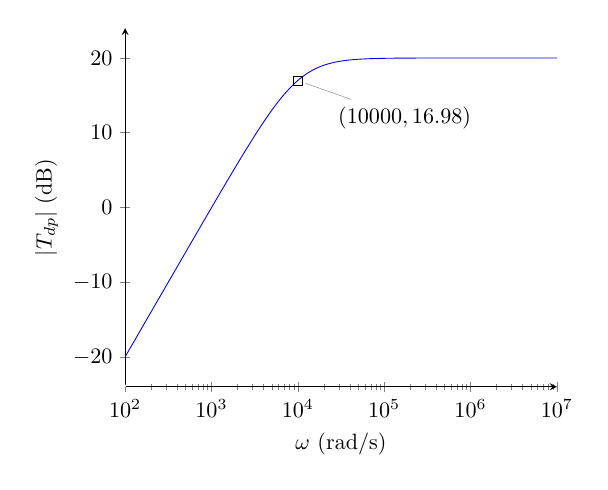
\begin{tikzpicture} [scale=0.8]
\begin{semilogxaxis}[
    axis lines = left,
    xlabel = {$\omega$ (rad/s)},
    ylabel = {$|T_{dp}|$ (dB)}
]
\addplot [
    domain=100:1000000, 
    samples=100, 
    color=white,
]
{24*log10(10*x/sqrt(x^2+(10000)^2))};
\addplot [
    domain=100:10000000, 
    samples=100, 
    color=blue,
]
{20*log10(10*x/sqrt(x^2+(10000)^2))};
\addplot[mark=square] coordinates {(10000,16.98)} node[pin=-30:{$(10000,16.98)$}]{};
\end{semilogxaxis}
\end{tikzpicture}
\hspace{1cm}
\begin{tikzpicture} [scale=0.8]
\begin{semilogxaxis}[
    axis lines = left,
    xlabel = {$\omega$ (rad/s)},
    ylabel = {$\angle T_{dp} $ (°)},
    xtick={10,100,1000,10000,100000,1000000,10000000},
    ytick={-180, -135, -90},
]
\addplot [
    domain=10:10000000, 
    samples=100, 
    color=blue
]
{-180+atan(10000/x))};
\addplot[mark=square] coordinates {(10000,-135)} node[pin=220:{$(10000,135)$}]{};
\addplot [
    domain=10:10000000, 
    samples=100, 
    color=white
]
{-90};
\addplot [
    domain=10:10000000, 
    samples=100, 
    color=white
]
{-180};
\end{semilogxaxis}
\end{tikzpicture}
\end{center}
\caption{Curvas de bode teóricas da função de transferência do derivador.}
\label{bode:2} 
\end{figure}

Se injetado um sinal quadrado no derivador cujo o espectro de frequência possui harmônicas, pode-se perceber que de acordo com que a faixa de frequências de maior potência fique a frequências abaixo da de corte, haverá uma intensa derivação do sinal, resultando em impulsos na saída. Porém, de acordo com que as frequências do sinal aumentem, elas enfrentarão a região de ganho constante, ficando sujeitas a não mais serem derivadas.

\section{Resultados e discussão}

Para encontrar todos os resultados necessários para comprovar a teoria, a prática foi dividida em algumas etapas, sendo elas:


\begin{itemize}

    \item Montar o circuito da figura \ref{ckt:1} e aplicar $V_{in} = sen (2\pi \times f_i \times t)$ V, variando-se $f_i$ de modo a se obter as curva de magnitude e ganho desse circuito;
    \item Realizar o mesmo procedimento no circuito da figura \ref{ckt:2};
    \item Aplicar um onda quadrada na entrada e comparar valores na frequência corte, muito abaixo da frequência de corte e muito superior a frequência de corte para ambos os circuito e verificar o que ocorre;
\end{itemize}

Para a obtenção das curvas de magnitude e fase dos circuitos da figura \ref{ckt:1} e \ref{ckt:2}, foi aplicado na entrada uma tensão de $V_{in} = sen (2\pi \times f_i \times t)$ V, variando o $f_{i}$ nas frequências de 1Hz a 100kHz, e também, na frequência de corte real dos circuitos. Foi possível obter os valores listados na tabela da figura \ref{table} encontrada no anexo, para ambos os circuitos, tanto o integrativo quanto o diferencial.

A frequência de corte para cada circuito foi determinada a partir do ângulo de defasagem entre entrada e saída, sendo de 135° para  o circuito integrador encontrando uma frequência de corte de $f_{oi} \approx 1,1kHz$, e -135° para o circuito diferenciador encontrando uma frequência de corte de $f_{od} \approx 1,75kHz$. Os  gráficos referentes a medição da fase e amplitude nas frequências de corte no osciloscópio se encontram podem ser observadas na figura \ref{cut}.

\begin{figure}[H] 
\centering
\subfigure[ref1][Integrador.]{\includegraphics[width=7.5cm]{imagens/f0_int.png}}
\subfigure[ref2][Derivador.]{\includegraphics[width=7.5cm]{imagens/f0_der.png}}
\caption{Forma de onda para entrada (CH2) e saída (CH1) na frequência de corte de cada circuito.}
\label{cut}
\end{figure}

Pode-se ainda visualizar os diagramas de fase e amplitude utilizando os valores encontrados na tabela da figura \ref{table} que se encontra em anexo. Dessa forma pode-se comparar as curvas de bode práticas com as teóricas e perceber que de fato há uma relação entre teoria e prática.

\begin{figure}[H]
\begin{center}
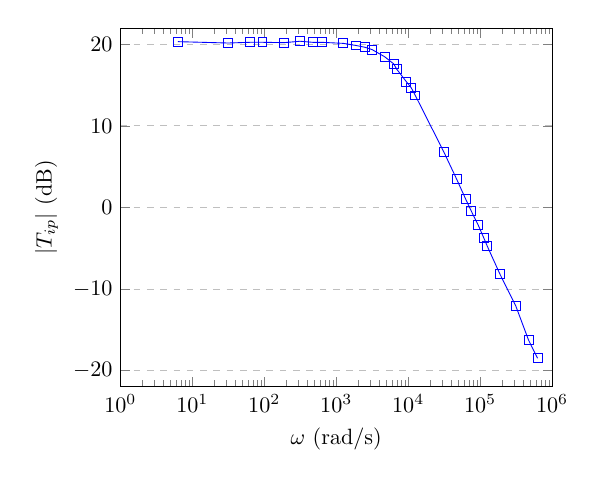
\begin{tikzpicture} [scale=0.8]
\begin{semilogxaxis}[
    title={},
    xlabel={$\omega$ (rad/s)},
    ylabel={$|T_{ip}|$ (dB)},
    xmin=1, xmax=1000000,
    ymin=-22, ymax=22,
    xtick={1,10,100,1000,10000,100000,1000000},
    ytick={-20,-10,0,10,20},
    legend pos=north west,
    ymajorgrids=true,
    grid style=dashed,
]
\addplot[
    color=blue,
    mark=square,
    ]
    coordinates {
    (6.28,20.339)
    (31.42,20.172)
    (62.83,20.259)
    (94.25,20.261)
    (188.5,20.217)
    (314.16,20.388)
    (471.24,20.257)
    (628.32,20.257)
    (1256.64,20.129)
    (1884.96,19.869)
    (2513.27,19.645)
    (3141.59,19.37)
    (4712.39,18.486)
    (6283.19,17.616)
    (6911.5,16.975)
    (9424.78,15.43)
    (10995.57,14.698)
    (12566.37,13.739)
    (31415.93,6.776)
    (47123.89,3.478)
    (62831.85,1.038)
    (75398.22,-0.45)
    (94247.78,-2.183)
    (113097.34,-3.789)
    (125663.71,-4.751)
    (188495.56,-8.18)
    (314159.27,-12.128)
    (471238.9,-16.28)
    (628318.53,-18.503)
    };
\end{semilogxaxis}
\end{tikzpicture}
\hspace{1cm}
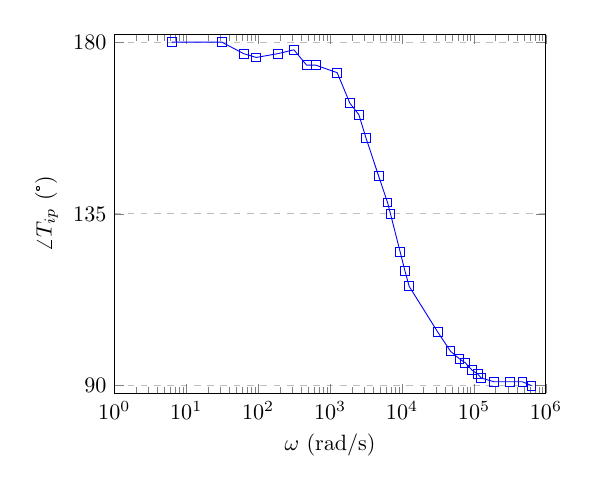
\begin{tikzpicture} [scale=0.8]
\begin{semilogxaxis}[
    title={},
    xlabel={$\omega$ (rad/s)},
    ylabel={$\angle T_{ip}$ (°)},
    xmin=1, xmax=1000000,
    ymin=88, ymax=182,
    xtick={1,10,100,1000,10000,100000,1000000},
    ytick={90, 135, 180},
    legend pos=north west,
    ymajorgrids=true,
    grid style=dashed,
]
\addplot[
    color=blue,
    mark=square,
    ]
    coordinates {
    (6.28,180)
    (31.42,180)
    (62.83,177)
    (94.25,176)
    (188.5,177)
    (314.16,178)
    (471.24,174)
    (628.32,174)
    (1256.64,172)
    (1884.96,164)
    (2513.27,161)
    (3141.59,155)
    (4712.39,145)
    (6283.19,138)
    (6911.5,135)
    (9424.78,125)
    (10995.57,120)
    (12566.37,116)
    (31415.93,104)
    (47123.89,99)
    (62831.85,97)
    (75398.22,96)
    (94247.78,94)
    (113097.34,93)
    (125663.71,92)
    (188495.56,91)
    (314159.27,91)
    (471238.9,91)
    (628318.53,90)
    };
\end{semilogxaxis}
\end{tikzpicture}
\end{center}
\caption{Curvas de bode com os resultados práticos da função de transferência do integrador.}
\label{graph:1} 
\end{figure}
\begin{figure}[H]
\begin{center}
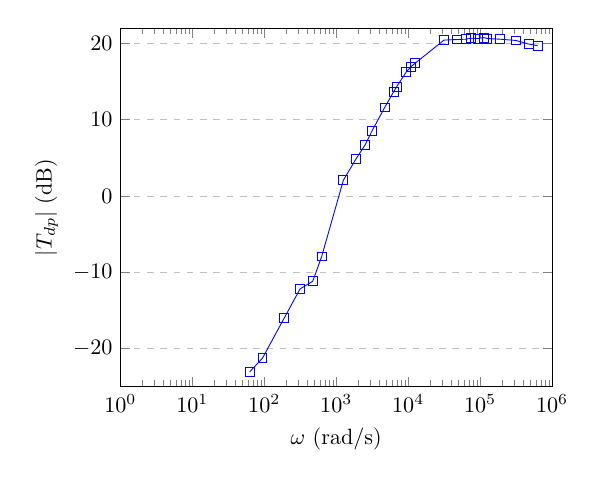
\begin{tikzpicture} [scale=0.8]
\begin{semilogxaxis}[
    title={},
    xlabel={$\omega$ (rad/s)},
    ylabel={$|T_{dp}|$ (dB)},
    xmin=1, xmax=1000000,
    ymin=-25, ymax=22,
    xtick={1,10,100,1000,10000,100000,1000000},
    ytick={-20,-10,0,10,20},
    legend pos=north west,
    ymajorgrids=true,
    grid style=dashed,
]
\addplot[
    color=blue,
    mark=square,
    ]
    coordinates {
    (62.83,-23.036)
    (94.25,-21.26)
    (188.5,-16.027)
    (314.16,-12.181)
    (471.24,-11.182)
    (628.32,-7.915)
    (1256.64,2.067)
    (1884.96,4.867)
    (2513.27,6.676)
    (3141.59,8.519)
    (4712.39,11.598)
    (6283.19,13.654)
    (6911.5,14.32)
    (9424.78,16.258)
    (10995.57,16.964)
    (12566.37,17.415)
    (31415.93,20.428)
    (47123.89,20.506)
    (62831.85,20.547)
    (75398.22,20.678)
    (94247.78,20.634)
    (113097.34,20.759)
    (125663.71,20.634)
    (188495.56,20.547)
    (314159.27,20.382)
    (471238.9,19.914)
    (628318.53,19.697)
    };
\end{semilogxaxis}
\end{tikzpicture}
\hspace{1cm}
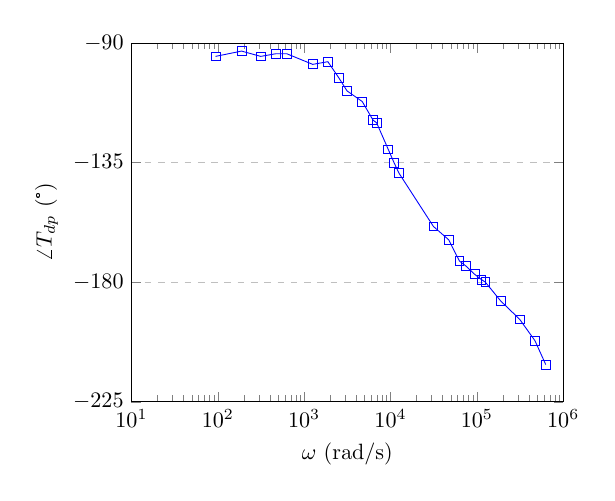
\begin{tikzpicture} [scale=0.8]
\begin{semilogxaxis}[
    title={},
    xlabel={$\omega$ (rad/s)},
    ylabel={$\angle T_{dp}$ (°)},
    xmin=10, xmax=1000000,
    ymin=-225, ymax=-90,
    xtick={10,100,1000,10000,100000,1000000},
    ytick={-225, -180, -135, -90},
    legend pos=north west,
    ymajorgrids=true,
    grid style=dashed,
]
\addplot[
    color=blue,
    mark=square,
    ]
    coordinates {
    (94.25,-95)
    (188.5,-93)
    (314.16,-95)
    (471.24,-94)
    (628.32,-94)
    (1256.64,-98)
    (1884.96,-97)
    (2513.27,-103)
    (3141.59,-108)
    (4712.39,-112)
    (6283.19,-119)
    (6911.5,-120)
    (9424.78,-130)
    (10995.57,-135)
    (12566.37,-139)
    (31415.93,-159)
    (47123.89,-164)
    (62831.85,-172)
    (75398.22,-174)
    (94247.78,-177)
    (113097.34,-179)
    (125663.71,-180)
    (188495.56,-187)
    (314159.27,-194)
    (471238.9,-202)
    (628318.53,-211)
    };
\end{semilogxaxis}
\end{tikzpicture}
\end{center}
\caption{Curvas de bode com os resultados práticos da função de transferência do derivador.}
\label{graph:2} 
\end{figure}


Podemos notar que limitações do circuito derivador e também pelas próprias limitações do CI LF353 e equipamentos utilizados, não se foi possível encontrar os valores de amplitude e fase para pequenos frequências, como 1Hz e para frequências acima de 100kHz. Acima de 100kHz o circuito apresentou um queda do ganho e da fase devido às limitações do CI, sendo eles oriundos da característica passa-baixa da função de transferência do próprio amplificador operacional não ideal. 

Para a segunda parte da atividade foi comparada a saída a partir de uma entrada quadrada com três diferentes frequências, onde $f_1<<f_{c}$, $f_2 = f_{c}$ e por fim $f_1>>f_{c}$. Para ambos os circuitos tanto o integrativo quanto o diferencial.

Primeiramente para o circuito integrador prático foram escolhidos frequências de 100 Hz, 10kHz, 850khz para serem comparadas com a frequência de corte do integrador $f_{ci} = 1,1 kHz$. Obteve-se as imagens abaixo:


\begin{figure}[H] 
\centering
\subfigure[ref1][100Hz.]{\includegraphics[width=7.5cm]{imagens/1_2_a.png}}
\subfigure[ref2][1.1kHz.]{\includegraphics[width=7.5cm]{imagens/1_2_b.png}}
\subfigure[ref3][10kHz.]{\includegraphics[width=7.5cm]{imagens/1_2_c.png}}
\subfigure[ref4][850kHz.]{\includegraphics[width=7.5cm]{imagens/1_2_d.png}}
\caption{Forma de onda para uma entrada na forma de uma onda quadrada (CH2) e saída (CH1) para diferentes frequências no circuito integrador.}
\end{figure}

Pode-se notar que para valores muito menores que a frequência de corte, o sinal de saída quase não sofre modificações por meio de uma integração, porém apenas uma ganho. Como todo sinal real é limitado no tempo, logo possui um espectro de frequência ilimitado, mesmo com a frequência principal em baixos valores, as harmônicas de alta frequência estarão na zona de integração, assim permitindo uma leve integração do sinal.

Já para valores na frequência de corte o circuito é integrado e multiplicado com os valores do inverso da constante de tempo, o que faz o circuito carregar e descarregar completamente, como pode ser observado na figura.

Para valores na faixa de 100kHz, tem-se o sinal de entrada integrado na saída com uma atenuação e por fim, para muito acima da frequência de corte a saída praticamente não tem ganho, pois seus valores são fortemente atenuados, mas ainda se percebe que o sinal é integrado.

Já para o circuito diferenciador foram escolhidos frequências de 100 Hz, 10kHz, 100khz para serem comparadas com a frequência de corte do integrador $f_{cd} = 1,75 kHz$. Obtemos asimagens abaixo:

\begin{figure}[H] 
\centering
\subfigure[ref1][100Hz]{\includegraphics[width=7.5cm]{imagens/2_2_a.png}}
\subfigure[ref2][1,75kHz]{\includegraphics[width=7.5cm]{imagens/2_2_b.png}}
\subfigure[ref3][10kHz]{\includegraphics[width=7.5cm]{imagens/2_2_c.png}}
\subfigure[ref4][100kHz]{\includegraphics[width=7.5cm]{imagens/2_2_d.png}}
\caption{Forma de onda para uma entrada na forma de uma onda quadrada (CH2) e saída (CH1) para diferentes frequências no circuito integrador.}
\end{figure}

A partir das imagens acima, para um circuito diferenciador prático, percebe-se para frequências muito menores que a de corte a atenuação é muito grande, já para a frequência de corte o circuito se comporta como o negativo da constante de tempo (RC) multiplicada pelo o sinal derivado da entrada dessa forma temos um decaimento na saída com a saturação dos no trem de pulsos. Já para valores muito acima da frequência de corte, teremos que o capacitor se comportará como aproximadamente um curto, logo teremos um circuito praticamente inversor, de modo que a saída é bem próxima a onda quadrada invertida.   

Pode-se perceber que na figura (a) o capacitor descarrega completamente. Já na figura (b), ele quase ainda possui um pouco de carga (na frequência de corte deveria descarregar completamente em um semi-período). Para a figura (c) já não há mais tempo para descarregar. Isso mostra que a constante de tempo RC permanece a mesma para o circuito, independentemente da frequência de entrada.




\section{Conclusões}

A prática foi de essencial importância para a confirmação dos valores teóricos do integrador e derivador, abrindo espaço para novas aplicações de circuitos analógicos com amplificadores operacionais. Também foi possível entender os limites físicos dos circuitos integrados utilizados, que por mais que são aproximadamente ideais, ainda possuem uma limitação no que confere a banda de passagem limitada dos amplificadores operacionais do CI LF353. Dessa forma, mesmo com as limitações de projeto, é possível compreender a importância desses circuitos, apresentando uma alternativa de alta velocidade na resposta e pela facilidade de implementação do circuito.





\newpage

\section{Anexos}

\begin{figure}[H] 
\includegraphics[scale=0.22]{imagens/calc1.jpg} 
\centering
\caption{Folha 1 de cálculos da prática.}
\label{p5-2} 
\end{figure} 

\begin{figure}[H] 
\includegraphics[scale=0.15]{imagens/calc2.jpg} 
\centering
\caption{Folha 2 de cálculos da prática.}
\label{p5-2} 
\end{figure} 

\newpage
\begin{figure}[h!]
	\centering
		\includepdf[page={1}]{table.pdf} 
	\caption{Tabela contendo os valores medidos na prática para ambos os circuitos.}
	\label{table}
\end{figure}











